\documentclass[12pt]{article}
\usepackage{amsmath,amssymb,graphicx}
\usepackage{geometry}
\geometry{margin=1in}
\usepackage{tikz}
\usetikzlibrary{arrows.meta,positioning,calc}
\title{Neuroplasticity in Multiplicity Theory: A Formal Overview}
\author{Citizen Gardens Research Network}
\date{September 2025}

\begin{document}

\maketitle

\section*{Overview}
This document formalizes the neuroplasticity framework within the broader paradigm of Multiplicity Theory, using the constructs of Recursive Operators $\Xi(t)$, Prime-Indexed Recursive Tensor Mathematics (PIRTM), and Consciousness Stability Law (CSL).

\section{Recursive Cognition and Prime Indexing}
Learning is modeled as a self-updating recursive function:
\begin{equation}
\Theta(t+1) = \Xi(\Theta(t))
\end{equation}

Cognitive states are encoded using prime-indexed tensors:
\begin{equation}
\Psi(t) = \sum_{p\,\in\,\mathbb{P}} \theta_p(t) \otimes e^{i\phi_p(t)}
\end{equation}
where $\theta_p(t)$ is the embodied cognitive trace, and $\phi_p(t)$ is the attention phase.

\section{Neuroquantum Interface}
Neuroplastic changes are interpreted as frequency-domain shifts:
\begin{equation}
\text{EEGLearn}(t) = \mathcal{F}^{-1}(\langle \psi | \hat{H} | \phi \rangle)
\end{equation}
This implies that recursive learning maps to Hermitian evolution filtered through subjective readiness.

\section{Ethical Constraints via CSL}
Emotional coherence must be conserved:
\begin{equation}
\Delta S < \ln \varphi
\end{equation}
where $\varphi$ is the golden ratio. This constraint prevents psychological overload, and supports trauma-aware, dignity-preserving change.

\section{Echo Braid: ASD-Centric Neuroplasticity}
In ASD-aligned models, recursive identity states are braided over primes:
\begin{equation}
\text{EchoBraid}(t) = \bigoplus_{n=1}^{\infty} \psi_{p_n}(t) \otimes e^{i\theta_{p_n}(t)}
\end{equation}
This enables phase-stable neuroplasticity across emotional and cognitive domains.

\section{Diagram: Neuroplastic Learning Loop}
\begin{center}
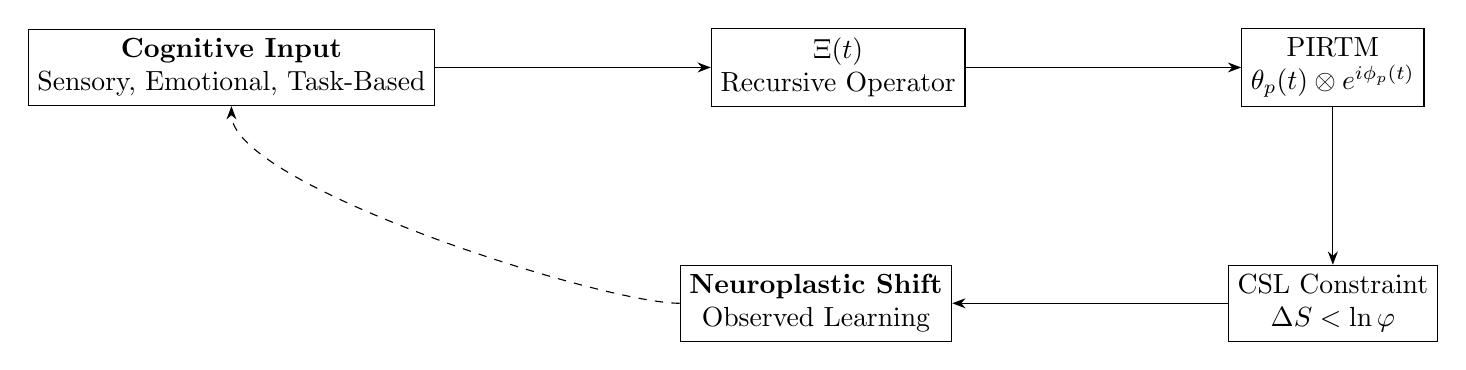
\begin{tikzpicture}[>=Stealth, node distance=2cm and 3.5cm, every node/.style={align=center}]
  \node (input) [rectangle, draw] {\textbf{Cognitive Input}\\Sensory, Emotional, Task-Based};
  \node (rec) [rectangle, draw, right=of input] {$\Xi(t)$\\Recursive Operator};
  \node (tensor) [rectangle, draw, right=of rec] {PIRTM\\$\theta_p(t) \otimes e^{i\phi_p(t)}$};
  \node (csl) [rectangle, draw, below=of tensor] {CSL Constraint\\$\Delta S < \ln \varphi$};
  \node (output) [rectangle, draw, left=of csl] {\textbf{Neuroplastic Shift}\\Observed Learning};

  \draw[->] (input) -- (rec);
  \draw[->] (rec) -- (tensor);
  \draw[->] (tensor) -- (csl);
  \draw[->] (csl) -- (output);
  \draw[->, dashed] (output.west) .. controls +(left:1cm) and +(down:1cm) .. (input.south);
\end{tikzpicture}
\end{center}

\section*{Conclusion}
This framework shows how lawful recursion, tensor encoding, and ethical bounds produce a formal and adaptive model of neuroplasticity that supports diverse, trauma-aware learning paths.

\end{document}